模拟量子系统有多种方法。例如，可以使用全状态矢量模拟纯态量子系统，也可以使用密度矩阵模拟混态量子系统。\MindQuantum\ 同时支持这两种方法。

\begin{lstlisting}
from mindquantum.core.gates import H
from mindquantum.simulator import Simulator

sim = Simulator('mqvector', 2)
sim.apply_gate(H.on(0))
print(sim)
\end{lstlisting}
输出为：

\begin{lstlisting}[escapeinside={\[}{\]}]
mqvector simulator with 2 qubits (little endian), dtype: mindquantum.complex128.
Current quantum state:
[$\surd{}$]2/2|00>
[$\surd{}$]2/2|01>
\end{lstlisting}

在上述示例中，我们初始化了一个名为 \code{"mqvector"} 的全状态矢量模拟器，它是一个全态量子模拟器。截至 0.9.0 版本，\MindQuantum\ 支持的所有模拟器如下表所示：
\begin{table}[ht]
    \begin{tabular}{ccccc}
        \toprule
        名称          & CPU & GPU & Complex64 & Complex128 \\
        \midrule
        mqvector      & 是  & 否  & 是        & 是         \\
        mqvector\_gpu & 否  & 是  & 是        & 是         \\
        mqmatrix      & 是  & 否  & 是        & 是         \\
        \bottomrule
    \end{tabular}
    \caption{支持的量子模拟器。}
    \label{tab:simulator_supported}
\end{table}
施加 Hadamard 门后，我们得到量子态 $\left(\ket{00}+\ket{01}\right)/\sqrt{2}$。需要强调的是，在整个框架中，我们使用小端序表示法；也就是说，对于基态 $\ket{01}$，第一个量子比特处于 $\ket{1}$ 态，第二个量子比特处于 $\ket{0}$ 态。

\MindQuantum\ 中的每个模拟器都维护一个量子态。我们可以使用以 \code{apply} 开头的方法改变量子态，也可以使用以 \code{get} 开头的方法从量子态中提取信息。

\subsubsection{\texttt{apply} 方法}

\code{apply} 方法会将某个算符施加到模拟器维护的量子态上，并改变该量子态。我们可以施加单个量子门、量子线路，也可以施加哈密顿量来操控量子态。需要注意的是，施加哈密顿量后，量子态不一定仍是规范归一的量子态。

\begin{lstlisting}
from mindquantum.core.circuit import Circuit
from mindquantum.core.operators import Hamiltonian, QubitOperator
from mindquantum.simulator import Simulator

circ = Circuit().h(0).x(1, 0)
ham = Hamiltonian(QubitOperator('X0 Y1'))
sim = Simulator('mqvector', 2)
sim.apply_hamiltonian(ham)
sim.apply_circuit(circ)
\end{lstlisting}
输出为：
\begin{lstlisting}[escapeinside={\[}{\]}]
mqvector simulator with 2 qubits (little endian), dtype: mindquantum.complex128.
Current quantum state:
-[$\surd{}$]2/2j|01[$\rangle$]
[$\surd{}$]2/2j|10[$\rangle$]
\end{lstlisting}

\subsubsection{\texttt{get} 方法}

\code{get} 方法不会改变模拟器维护的量子态，而是从中提取有用信息。

- \getqs：可以通过该方法从模拟器中获取量子态向量，或在传入参数 \code{ket=True} 时获取 ket 字符串表达式。
\begin{lstlisting}
from mindquantum.algorithm.library import qft
from mindquantum.simulator import Simulator

sim = Simulator('mqvector', 3)
sim.apply_circuit(qft(range(3)))
qs = sim.get_qs()
print(sim.get_qs(ket=True))
\end{lstlisting}

- \getexpectation：计算给定可观测量的期望值是非常常见的需求。在 \MindQuantum\ 中，我们将可观测量的定义扩展为如下形式：

\begin{equation}
    E = \bra{\varphi}U_l^\dagger H U_r \ket{\psi}.
\end{equation}

根据该定义，如果设置 $\ket{\varphi}=\ket{\psi}$ 且 $U_l = U_r$，就可以方便地得到物理可观测量；如果设置 $H=I$，也可以计算两个量子态之间的内积。

\begin{lstlisting}
from mindquantum.core.circuit import Circuit
from mindquantum.core.operators import Hamiltonian, QubitOperator

# 获取期望值
psi = Simulator('mqvector', 2)
H = Hamiltonian(QubitOperator("Z0 Z1"))
U_r = Circuit().rx(2.5, 0)
print("Expectation:", psi.get_expectation(H, U_r))

# 获取内积
phi = Simulator("mqvector", 2)
H = Hamiltonian(QubitOperator(""))
U_l = Circuit().ry(1.5, 0)
print("Inner product:")
print(psi.get_expectation(H, U_r, U_l, phi))
\end{lstlisting}
输出为：

\begin{lstlisting}
Expectation: (-0.8011436155469336+0j)
Inner product:
(0.23071786267161518-0.6468646992187576j)
\end{lstlisting}

\subsubsection{采样}

量子采样是量子计算的基础内容之一，在高效求解某些复杂问题时发挥着关键作用。它利用量子叠加和纠缠原理同时探索多种可能性，使量子计算机能够在特定场景下超越经典计算机。

在 \MindQuantum\ 中，可以使用模拟器对量子线路的测量结果进行采样。
\begin{lstlisting}
from mindquantum.utils import random_circuit
from mindquantum.simulator import Simulator

circ = random_circuit(3, 5, seed=42)
circ.barrier().measure_all()
sim = Simulator('mqvector', circ.n_qubits)
res = sim.sampling(circ, shots=1000, seed=42)
\end{lstlisting}

\begin{figure}[h]
    \begin{center}
        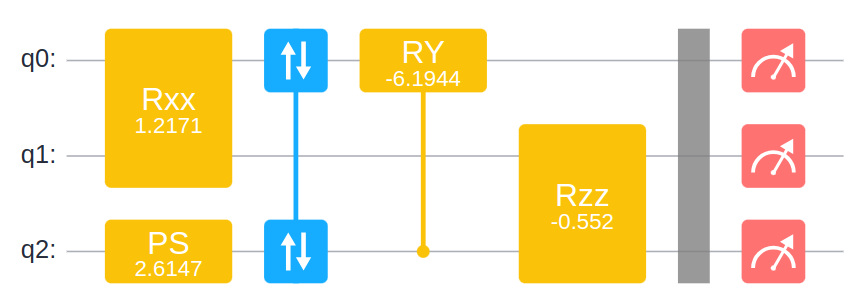
\includegraphics[width=0.9\linewidth]{images/2_6_sampling_circ.png}
    \end{center}
    \caption{采样线路}
\end{figure}

\begin{figure}[h]
    \begin{center}
        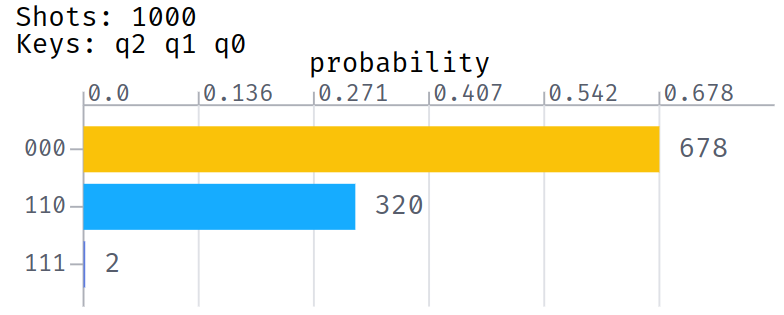
\includegraphics[width=0.9\linewidth]{images/2_6_sampling_res.png}
    \end{center}
    \caption{采样结果}
\end{figure}
